\chapter{Zbiór danych}

% pamiętać, żeby opisać wszystkie kroki, wszystkie SKRYPTY (koncepcję i algorytmy opisać szczegółowo,
% szczegóły techniczne, jak co zwraca, co przyjmuje dana funkcja pominąć), zerknąć na COMMITY

% potrzeba danych!
Pierwszym i jednocześnie najważniejszym etapem w tworzeniu rozwiązania opartego o uczenie maszynowe
jest zgromadzenie odpowiedniego zbioru danych. Jest to etap kluczowy, co wydaje się oczywiste po
uwzględnieniu natury tychże algorytmów --- wynajdują one pewne reguły na bazie podanych przykłady.

% potrzeba danych oznaczonych (jak zawsze) i nieoznaczonych (bo pomogą a są)
Głęboki sieci neuronowe, co do zasady potrzebują ,,dużo'' (zazwyczaj wiele milionów) przykładów
uczących, aby móc znaleźć poprawne reguły i wzorce --- aby nauczyć się odpowiedniej ekstrakcji cech. W
celu wytrenowania sieci do konkretnego zadania (np. do klasyfikacji obrazów), potrzeba zbioru
zawierającego dane wejściowe do modelu i oczekiwane dane wyjściowe z modelu. Takie uczenie na
podstawie przykładów oznaczonych (ze znaną wartością oczekiwaną) to \emph{uczenie nadzorowane}. Często jednak
ilość danych oznaczonych jest ograniczona, można wtedy wykorzystać dane bez oznaczeń w różnych
algorytmach \emph{uczenia nienadzorowanego}, aby nauczyć sieć struktury tych danych, bez
ukierunkowania na konkretne zadanie. Dopiero później wykorzystuje się mniejszą ilość danych
oznaczonych, aby dotrenować sieć (ang. \emph{finetuning}) i nauczyć ją rozwiązywać dany problem.

% co zawiera ten rozdział - od szukania danych do wejścia do sieci + opis skryptów
W ramach niniejszej pracy, ze względu na ograniczoną ilość danych oznaczonych, zastosowane zostało
właśnie powyższe podejście. Do przeprowadzenia eksperymentów potrzebne były dwa zbiory: pierwszy to
,,niewielki'' zbiór danych oznaczonych a drugi to ,,zdecydowanie większy'' zbiór danych bez
oznaczeń. W tym rozdziale opisany został proces pozyskiwania obu zbiorów danych z ogólnie
dostępnych źródeł. Zawarto tutaj opis wszystkich kroków wykonanych w celu przygotowania danych do
treningu sieci, poczynając od wyszukiwania oznaczeń utworów muzycznych i przygotowanie parsera dla
plików z tymi oznaczeniami, poprzez automatyczne wyszukiwania i pobieranie odpowiednich plików z
nagraniami muzycznymi, aż po wstępne przetwarzanie danych do formatu odpowiedniego dla sieci
neuronowej. Dodatkowo rozdział ten, poza opisem zastosowanych rozwiązań, zawiera również ogólny opis
implementacji tychże rozwiązań, którą to implementację stanowią skrypty języka Python.

% od początku do uzyskania wszystkich oznaczeń ('data/chordlab') oraz pierwszego indeksu (skrypt 01)
\section{Pozyskanie zbiorów danych z oznaczeniami akordów}

% trudno o dane oznaczone w ACR
Ze względu na powszechną dostępność dużej ilości danych w Internecie, zgromadzenie zbioru danych
nieoznaczonych nie stanowiło szczególnego problemu. Znacznie trudniejsze okazało się zgromadzenie
zbioru danych oznaczonych. Zadanie rozpoznawania akordów muzycznych, mimo iż będące jednym z
głównych zadań z dziedziny MIR, jest oczywiście bardzo mało popularne w stosunku do takich
zadań jak klasyfikacja, czy segmentacja obrazów. Jest to również po prostu znacznie mniej przydatne
w życiu codziennym i znacznie mniej się w tę dziedzinę inwestuje. Ponadto przygotowanie oznaczeń
akordów do utworów muzycznych wymaga specjalistycznej wiedzy muzycznej, praktyki muzycznej i dużo
czasu. Oznaczenia powstałe w ten sposób nadal pozostają subiektywne i będą się często różnić, w
zależności od osoby, która utwory oznaczała. Wszystkie wymienione powody są przyczyną tego, że nie
przygotowano więcej niż kilka publicznie dostępnych zbiorów oznaczeń akordów muzycznych, które mogą
zostać wykorzystane do treningu modeli uczenia maszynowego.

% zbiory są takie, co to inni wykorzystywali
W ramach niniejszej pracy przestudiowana została literatura z dziedziny rozpoznawania akordów za
pomocą sieci neuronowych --- większość wykorzystywanych przez badaczy zbiorów danych udało się
odnaleźć i wykorzystać. Zostały one szczegółowo opisane poniżej. Każdy zbiór oznaczeń został
pobrany, odpowiednio oczyszczony (wybrane zostały tylko niezbędne pliki) i zapisany w repozytorium
projektu (w katalogu \url{data/chordlab}). Po przeanalizowaniu struktury zbiorów stworzony został
pierwszy skrypt przygotowujący dane --- \url{src/dataset\_scripts/01-generate\_index\_of\_chordlab.py} ---
który, w postaci pliku \filetype{csv}, generuje jeden wspólny indeks (\url{data/index.csv}) dla wszystkich
zbiorów, tak że mogą one być już traktowane jako jeden zbiór danych. Fragment tego indeksu został
przedstawiony w \ref{tab:indeks_01}.

\begin{table}
    \centering
    \caption{Fragment indeksu zbioru danych po pierwszym etapie jego tworzenia.}
    \label{tab:indeks_01}
    \makebox[\textwidth][c]{
    {\scriptsize \ttfamily \begin{tabular}{rllllr}
    \hline
    & filepath & song & artist & subset & album \\
    \hline
     0 & ./data/\ldots/1999\_dt.clt                      & 1999                      & Prince                      & rs200 & nan \\ 
     1 & ./data/\ldots/a\_change\_is\ldots & A Change Is Gonna Come    & Sam Cooke                   & rs200 & nan \\
     5 & ./data/\ldots/all\_along\_t\ldots & All Along the Watchtower  & The Jimi Hendrix Experience & rs200 & nan \\
     6 & ./data/\ldots/all\_apologie\ldots & All Apologies             & Nirvana                     & rs200 & nan \\
     7 & ./data/\ldots/all\_i\_have\ldots & All I Have to Do Is Dream & The Everly Brothers         & rs200 & nan \\
    \hline
    \end{tabular}}}
\end{table}

Trzeba jeszcze zaznaczyć, że wszystkie te zbiory są udostępniane za darmo, ale jedynie jako same
pliki tekstowe z oznaczeniami akordów. Pliki z nagraniami muzycznymi, ze względu na prawa autorskie,
nie są udostępniane. Pozyskanie odpowiednich nagrań stanowi osobny problem, opisany w dalszej części
rozdziału.

\subsection{Zbiór Isophonics}

% ogólny opis, jakie i ile utworów, format zapisu
\emph{Isophonics} to właściwie nazwa serwisu internetowego\footnote{www.isophonics.net/about},
prowadzonego przez zespół naukowy \emph{Centre for Digital Music} z londyńskiego Uniwersytety
Królowej Marii. Jest to duża i popularna na cały świat jednostka naukowa specjalizująca się w
badaniach dotyczących przetwarzania muzyki cyfrowej. W serwisie tym dostępne są między innymi
oprogramowanie oraz zbiory danych związane z różnymi aspektami przetwarzania sygnałów muzycznych.
Można tam znaleźć najbardziej popularny i zapewne najstarszy zbiór z oznaczeniami akordów
muzycznych, przygotowany dla 180 piosenek zespołu \emph{The Beatles}, szczegółowo opisany w
\cite{harte_towards_nodate}. Zbiór ten rozrósł się o oznaczenia dla 20 utworów \emph{Queen}, 18
utworów \emph{Zweieck} i 7 utworów \emph{Carole King}. Wykorzystany format zapisu oznaczeń akordów
również jest opisany w \cite{harte_towards_nodate} i jest wykorzystywany praktycznie jako standard,
również w przypadku innych zbiorów danych. Warto wspomnieć jeszcze, że jest to pierwszy referencyjny
zbiór wykorzystywany w konkursie MIREX, w zadaniu automatycznego rozpoznawania akordów.

% pobieranie i indeksowanie
Zbiór \emph{Isohponics} jest dostępny do pobrania ze strony projektu w postaci skompresowanych
archiwów \filetype{tar} (osobny plik dla każdego z czterech artystów). Każde z tych archiwów ma taką
samą strukturę i zawiera nie tylko oznaczenia akordów, dostępne w różnych formatach, ale również
inne informacje o utworach, jak zmiany tonacji czy segmentacje strukturalne. Spośród wszystkich tych
plików wykorzystane zostały jedynie oznaczenia akordów w postaci plików \filetype{lab} - pozostałe pliki
zostały usunięte. Pliki z oznaczeniami akordów uporządkowane są w takiej stukturze katalogów, gdzie
nazwy katalogów na kolejnych poziomach zagłębienia odpowiadają kolejno nazwie artysty, nazwie albumu
(dla The Beatles poprzedzonej dodatkowo liczbą porządkową) i numerowi wraz z nazwą konkretnego
utworu. Zbiór ten nie posiada żadnego dodatkowego indeksu, przy tworzeniu własnego indeksu zostały
więc wykorzystane nazwy katalogów.

% poprawki i zapisanie w projekcie
Jedyne zmiany, jakie zostały wprowadzone w oznaczeniach akordów po pobraniu ich z Internetu, poza
usunięciem niewykorzystywanych plików, dotyczą artystki Carole King. Polegały one na dostosowaniu
kilku skrótów typów akordów, które występowały jedynie tutaj a były niezgodne z przyjętą w
\cite{harte_towards_nodate} konwencją. Wszystkie oznaczenia zbioru \emph{isohponics}, po
przeprowadzeniu opisanych powyżej operacji, zostały zapisane w repozytorium projektu, w katalogu
\url{data/chordlab/isophonics}.


\subsection{Zbiór McGill Billboard}

% ogólny opis, jakie i ile utworów, format zapisu
Zbiór \emph{McGill Billboard} \cite{burgoyne_expert_2011} został stworzony przez grupę \emph{DDMAL
(Distributed Digital Music Archives \& Libraries Lab)}\footnote{https://ddmal.music.mcgill.ca/} z
kandadyjskiego \emph{McGill University}. Jak nazwa wskazuje, zajmują się oni różnymi projektami
związanymi z przetwarzaniem muzyki, w tym tworzą i utrzymują ten prawdopodobnie największy, dostępny
publicznie zbiór danych z różnymi typami oznaczeń utworów, takimi jak akordy, struktura, instrumenty
i tempo. Lista utworów wybranych do tego zbioru została zbudowana z 1300 utworów, losowo
próbkowanych z rankingów serwisu \emph{Billboard}\footnote{www.billboard.com}. W praktyce, ponieważ
niektórych utworów nie udało się twórcom znaleźć, zbiór ten zawiera 890 utworów muzyki popularnej,
przy czym zdarzają się takie, które się powtarzają. Oznaczenia akordów są wyrównane w czasie zgodnie
z częstotliwością występowania taktów. Format tych oznaczeń bazuje ściśle na
\cite{harte_towards_nodate} (tak jak \emph{isophonics}), jedyna różnica polega na wprowadzeniu kilku
dodatkowych skrótów typów akordów.  Podobnie jak w przypadku innych zbiorów z oznaczeniami akordów,
twórcy tego zbioru nie mogli udostępnić nagrań muzycznych. Jednakże w tym przypadku udostępnione
zostały dwa zestawy cech dla wszystkich akordów: \emph{non-negative-least-squares chroma vectors}
oraz \emph{Echo Nest features}, które mogą zostać wykorzystane jako wejście do modeli ML, nie były
jednak użyte w ramach niniejszej pracy.

% pobieranie i indeksowanie
Zbiór \emph{McGill Billboard} dostępny jest do
pobrania\footnote{https://ddmal.music.mcgill.ca/research/The\_McGill\_Billboard\_Project\_(Chord\_Analysis\_Dataset)/}
w postaci skompresowanych (na kilka sposobów) archiwów \filetype{tar}. Dostępne są pliki ze wspomnianymi
powyżej dwoma zestawami dźwiękowych cech utworów, dostępny jest zestaw wszystkich oznaczeń we
własnym formacie twórców zbioru, oraz zestaw oznaczeń samych akordów, w postaci plików \filetype{lab}.
Do niniejszej pracy wykorzystany został jedynie ten ostatni zestaw, zawierający pliki \filetype{lab}. Pobrane
archiwum zawiera główny katalog \url{McGill-Billboard}, w którym znajduje się 890 katalogów nazwanych
liczbowymi identyfikatorami utworów ze zbioru. Każdy taki katalog zawiera jeden plik \url{full.lab} z
oznaczeniami akordów. Twórcy zbioru dostarczają również indeks w postaci pliku \filetype{csv}, wiążący
identyfikatory utworów z tytułem, artystą (album nie jest podany) i innymi informacjami związanymi z
rankingiem, z którego pochodzi utwór. Indeks ten jest niestety bardzo wybrakowany i dla wielu
utworów brakuje wpisu o tytule lub artyście. Po wybraniu tych przypadków, dla których znany jest
tytuł i artysta zostało jedynie 596 utworów. Tabela ta została wykorzystana do przygotowanie
własnego indeksu.

% poprawki i zapisanie w projekcie
Pobrane oznaczenia akordów nie wymagały właściwie żadnych poprawek. Cały katalog
\url{McGill-Billboard} został przeniesiony do repozytorium projetu, do katalogu
\url{data/chordlab/mcgill\_billboard}.

\subsection{Zbiór Robbie Williams}

% ogólny opis, jakie i ile utworów, format zapisu
Zbiór \emph{Robbie Williams} \cite{giorgi_automatic_2013} składa się z oznaczeń akordów oraz tonacji
dla pierwszych pięciu albumów Robbiego Williamsa. Został przygotowany przez włoskich naukowców z
Politechniki w Mediolanie na potrzeby uczenia systemu automatycznego rozpoznawania akordów.
Oznaczenia są zgodne z \cite{harte_towards_nodate}. W sumie dokładne oznaczenia akordów i tonacji
przygotowano dla 65 utworów.

% pobieranie i indeksowanie
Zbiór ten dostępny jest do pobrania ze strony
\footnote{https://www.researchgate.net/publication/260399240\_Chord\_and\_Harmony\_annotations\_of\_the\_first\_five\_albums\_by\_Robbie\_Williams}
w postaci archiwum zip. Znajduje się w nim katalog \url{RobbieWilliamsAnnotations}, który zawiera
dwa główne podkatalogi: \url{chords} i \url{keys}. W każdym z tych podkatalogów znajduje się po pięć
podkatalogów (po jednym na album). W każdym katalogu z albumem znajdują się pliki \emph{txt} z
oznaczeniami akordów w formacie \filetype{lab}. Zbiór ten nie posiada żadnych dodatkowych metadanych,
własny indeks wygenerowany został na podstawie znormalizowanych nazw katalogów.

% poprawki i zapisanie w projekcie
Pobrane oznaczenia znowu nie wymagały żadnych poprawek. Zawartość katalog
\url{RobbieWilliamsAnnotations/chords/} została przeniesiona do repozytorium projektu, do katalogu
\url{data/chordlab/robbie\_williams}.

\subsection{Zbiór RS200}

% ogólny opis, jakie i ile utworów, format zapisu
Zbiór \emph{RS200} \cite{de_clercq_corpus_2011} został stworzony przez dwóch badaczy z amerykańskiej
uczelni muzycznej \emph{Eastman School of Music} w Rochester. Powstał on na bazie listy \emph{500
Greatest Songs of All Time} z magazynu \emph{Rolling Stone}. Początkowo zawierał jedynie 100 utworów i w
takiej formie został wykorzystany w oryginalnej publikacji, gdzie autorzy analizowali częstość
występowania różnych akordów i ich progresji. Utwory te zostały wybrane tak, aby pochodziły z wielu
różnych dekad. Z czasem zbiór został rozszerzony do 200 utworów i w takiej formie jest dostępny do
dzisiaj. Każdy z dwóch twórców, niezależnie od drugiego, przygotował swoje oznaczenia dla wszystkich
200 utworów. Oznaczenia te zawierają nie tylko akordy, ale również transkrypcję melodii, informacje
o tempie i tekstach utworów. Format zapisu oznaczeń akordów został opracowanych przez twórców tego
zbioru danych i różni się zdecydowanie od sposobu oznaczeń stosowanego w pozostałych zbiorach.
Bardziej szczegółowo został opisany w dalszej części rozdziału, ale ogólnie opiera się on na
rekurencyjnej składni, pozwalającej łatwo reprezentować pewne schematy i powtórzenia w strukturze
utworów. Same oznaczenia akordów są również ustalone przez tych autorów i bazują na liczbach
rzymskich, które prezentują informacje względem tonacji całego utworu. Mamy więc tutaj do
czynienia z podejściem zupełnie innym, od przyjętego dla pozostałych zbiorów danych.

% pobieranie i indeksowanie
Zbiór ten dostępny jest do pobrania ze strony
\footnote{http://rockcorpus.midside.com/harmonic\_analyses.html}. Właściwie autorzy oferują trzy
formaty, z których ostatni jest już rozwinięty do postaci zbliżonej do plików \filetype{lab}. Główna
różnica to wspomniany powyżej sposób oznaczania konkretnych akordów. Po pobraniu i rozpakowaniu archiwum
\emph{zip} znaleźć można pojedynczy katalog \url{rs200\_harmony\_clt}, który zawiera pliki z
rozszerzeniem \emph{clt}, po dwa dla każdego utworu, jeden z suffiksem ,,dt' a drugi ,,tdc'' (od
nazwisk autorów). Ze względu na to, że oznaczenia jednego z autorów były znacznie bardziej
uporządkowane i prostsze a kwestia różnić w oznaczeniach dwóch różnych osób nie jest szczególnie
związana z tematem niniejszej pracy, wybrane zostały jedynie oznaczenia z sufikem ,,dt''. Jeżeli
chodzi o indeksowanie plików z oznaczeniami, to autorzy dostarczają plik \emph{txt} z opisem
wszystkich plików z oznaczeniami, w tym z tytułem utworu, rokiem wydania i nazwiskiem artysty. Plik
ten, po wprowadzeniu kilku niezbędnych poprawek (literówki i pomyłki w nazwach, odniesienia do
nieistniejących plików), został wykorzystany do generowania głównego indeksu utworów.

% poprawki i zapisanie w projekcie
Wybrane pliki z suffiksem ,,dt'' nie wymagały już więcej poprawek. Zostały wszystkie, przeniesione
do katalogu \url{data/chordlab/rs200}.

\subsection{Zbiór RWC POP}

% ogólny opis, jakie i ile utworów, format zapis
Zbiór RWC POP \cite{goto_rwc_nodate} stanowi część większego zbioru o nazwie RWC (Real World
Computing) Music Database\footnote{https://staff.aist.go.jp/m.goto/RWC-MDB/}, stworzonego przez Real
World Computing Partnership (RWCP) w Japonii. Jest to oczyszczony z praw autorskich, dostępny za
darmo (trzeba pokryć jedynie koszty kopiowania i dostawy) wielkoskalowy zbiór 315 utworów
muzycznych, podzielonych na 5 zestawów o różnym zastosowaniu, jak rozpoznawanie gatunku czy
instrumentu muzycznego. Jednym z tych zestawów jest właśnie Popular Music Database zawierający 100
utworów muzyki popularnej - 20 w stylu popularnej muzyki zachodniej z lat 80-tych (w języku
angielskim) i 80 w stylu popularnej muzyki japońskiej, z lat 90-tych (w języku japońskim). Właściwie
zbiór ten, poza potencjalną możliwością uzyskania darmowego i legalnego dostępu do nagrań
dźwiękowych, nie jest przydatny dla zadania rozpoznawania akordów, ponieważ nie zawiera oznaczeń
akordów. Te zostały jednak przygotowane dla wszystkich 100 utworów przez studentów uniwersytetu w
Nowym Jorku z Music and Audio Research Lab. Format tych oznaczeń jest ponownie zgodny z
\cite{harte_towards_nodate}. W ramach niniejszej pracy wykorzystane zostały właśnie te oznaczenia.
Dla uproszczenia i zautomatyzowania całego procesu przygotowania danych, nagrania muzyczne próbowano
pozyskać tą samą metodą jak w przypadku pozostałych zbiorów danych.

% pobieranie i indeksowanie
Oznaczenia akordów do zbioru RWC POP są dostępne za darmo do pobrania w Internecie jako repozytorium
git w serwisie GitHub\footnote{https://github.com/tmc323/Chord-Annotations}. Bezpośrednio w
repozytorium znajduje się katalog \url{RWC\_Pop\_Chords}, który zawiera pliki z oznaczeniami akordów w
dwóch formatach: \url{svl} oraz \filetype{lab}. Wykorzystane zostały jedynie pliki \filetype{lab}. Nazwy
tych plików zawierają liczbowe identyfikatory poszczególnych nagrań. Aby przygotować indeks i
pozyskać informacje o tytułach, nazwach albumów i nazwiskach artystów ze strony
projektu\footnote{https://staff.aist.go.jp/m.goto/RWC-MDB/rwc-mdb-p.html} skopiowana została tabela
ze wszystkimi tymi informacjami. Tabela ta zapisana została w pliku
\url{data/chordlab/rwc\_pop/rwc\_pop.txt} i była wykorzystana w skrypcie generującym indeks.

% poprawki i zapisanie w projekcie
Przygotowane przez nowojorskich studentów oznaczenia nie wymagały żadnych poprawek. Wszystkie pliki
\filetype{lab} zostały umieszczone w katalogu \url{data/chordlab/rwc\_pop}.

\subsection{Zbiór Uspop2002}

% ogólny opis, jakie i ile utworów, format zapis
Zbiór uspop2002 \cite{berenzweig_large-scale_2004} został przygotowany w ramach współpracy naukowców
z \emph{LabROSA (Laboratory for the Recognition and Organization of Speech and Audio)} z
Uniwersytetu w Kolumbii, naukowców z MIT i naukowców z \emph{HP Labs} w Cambridge. Jest to zbiór
8752 utworów, pochodzących od 400 różnych artystów, z 706 różnych albumów. Podobnie jak w przypadku
większości wykorzystanych zbiorów danych, oryginalne nagrania muzyczne nie są udostępniane
bezpośrednio - dostępne są jedynie wyekstrachowane wcześniej cechy MFCC. Zbiór ten został stworzony
na potrzeby badań nad miarami podobieństwa między utworami, autorzy nie dostarczają więc oznaczeń
akordów. Na szczęście studenci z Nowego Jorku, poza przygotowaniem oznaczeń dla zbioru RWC POP,
przygotowali również oznaczenia akordów dla 195 utworów z tego zbioru. Oznaczenia te mają ponownie
format plików \filetype{lab}, zgodny z \cite{harte_towards_nodate}. W ramach niniejszej pracy zbiór
uspop2002 nie był więc wykorzystywany bezpośrednio, a jedynie jako punkt wyjścia dla twórców
wspomnianych 195 plików z oznaczeniami, które to dopiero były wykorzystane w niniejszej pracy.

% pobieranie i indeksowanie
Dokładnie tak jak w przypadku zbioru RWC POP oznaczenia są dostępne za darmo do pobrania w
Internecie - stanowią część tego samego reozytorium w serwisie
GitHub\footnote{https://github.com/tmc323/Chord-Annotations}. Znajdują się w katalogu
\url{uspopLabels}, który zawiera katalogi nazwane nazwiskami artystów. Każdy z katalogów artysty
zawiera katalogi (zazwyczaj jeden) z nazwami albumów. Dopiero w katalogach z albumami znajdują się
pliki \filetype{lab}, zawierające w nazwie tytuły konkretnych utworów. Nazwy katalogów i nazwy plików
zostały wykorzystane podczas generowania indeksu.

% poprawki i zapisanie w projekcie
Ponownie oznaczenia nie wymagały żadnych poprawek. Całą zawartość katalogu \url{uspopLabels}
przeniesiono do katalogu projektu \url{data/chordlab/uspop}.

% duplikaty i podsumowanie
\subsection{Usuwanie duplikatów i podsumowanie pozyskanych oznaczeń}

Ostatnim etapem przygotowania wspólnego indeksu, opisującego wszystkie pozyskane pliki z
oznaczeniami, jest usunięcie duplikatów. Procedura ta, stanowiąca ostatni fragment skryptu
tworzącego indeks, jest następująca:

\begin{enumerate}
    \item Znormalizuj kolumny z nazwą utworu, artysty i albumu poprzez zamianę wszystkich wielkich
        liter na małe oraz usunięcie białych znaków z początku i końca ciągów tekstowych
    \item Pogrupuj wszystkie utwory po kluczu składającym się z tytułu i nazwy artysty, grupy te
        zawierają potencjalne duplikaty utworów
    \item Jeżeli w grupie występują razem utwory ze znanym albumem i bez albumu, to usuń wszystkie
        utwory bez albumu
    \item Jeżeli w grupie występuje kilka utworów z tym samym albumem, to zostaw tylko jeden
        (losowy) spośród nich
\end{enumerate}

W sumie wszystkich plików z oznaczeniami udało się zgromadzić 1380. Po etapie usuwania duplikatów
pozostało 1268. Tabela \ref{tab:datasets1} prezentuje rozkład wszystkich dostępnych plików z
oznaczeniami między poszczególne, opisane wcześniej zbiory danych.

\begin{table}
    \centering
    \caption{Liczebności plików z oznaczeniami dla poszczególnych zbiorów danych.}
    \label{tab:datasets1}
    \begin{tabular}{|l|c|c|c|c|c|c|c|} \hline
        Nazwa zbioru & Liczba utworów (z duplikatami) \\ \hline
        Isophonics & 225 (225) \\
        McGill Billboard & 509 (596) \\
        Robbie Williams & 65 (65) \\
        RS200 & 174 (199) \\
        RWC POP & 100 (100) \\
        Uspop2002 & 195 (195) \\
        SUMA & 1268 (1380) \\ \hline
    \end{tabular}
\end{table}


% annotation parser i implementacja WCSR
\section{Model akordów muzycznych i parsowanie plików z oznaczeniami} \label{section:chord_model}

% potrzeba parsowania - wstęp
Po zgromadzeniu, oczyszczeniu i zindeksowaniu zbiorów z oznaczeniami akordów, należało przygotować
skrypty parsujące pliki z tymi oznaczenia. Wszystkie znalezione zbiory oznaczeń, z wyjątkiem
jednego, są w formacie \filetype{lab}, który to format został opracowany w \cite{harte_towards_nodate}.
Jest to format bardzo przemyślany i dopracowany, którego użycie przez wielu niezależnych badaczy
potwierdza, że sprawdza się on jako standard. Drugi format, znacznie mniej usystematyzowany,
opracowany został na potrzeby zbioru RS200, gdzie autorzy przygotowali własny sposób oznaczania
akordów. Aby na końcu wykorzystać zarówno oznaczenia jak i nagrania muzyczne do treningu sieci
neuronowych, trzeba przetłumaczyć pliki tekstowe z oznaczeniami, na odpowiednią, zrozumiałą dla
komputera strukturę danych. W ramach tego podrozdziału opisana zostania najpierw ta struktura, a
następnie algorytm parsowania obu dostępnych formatów oznaczeń akordów. Skrypty pythonowe, które
realizują zadanie tłumaczenia oznaczeń w formacie plików tekstowych na odpowiednią strukturę danych,
umieszczone zostały w module \url{src/annotation\_parser}.

% Opis modelu akordu - skrypt chord_model.py
\subsection{Model obiektowy reprezentujący akordy muzyczne} \label{subsection:chord_model}

% Podstawowy model obiektowy akordu według Krzyśka
W ramach niniejszej pracy przygotowany został obiektowy model reprezentujący akord muzyczny. Model
ten ma formę zestawu klas pythonowy (w pliku \url{src/annotation\_parser/chord\_model.py}) i bazuje
ściśle na propozycji \cite{harte_towards_nodate}. Według oryginalnego pomysłu, każdy akord
reprezentowany jest przez trzy części składowe podstawę akordu (ang. \emph{root}), interwały
składowe (ang. \emph{component intervals}) oraz bas (ang. \emph{bass note}). Podstawa to po prostu
nazwa dźwięku, na którym akord jest zbudowany. Nazwa ta reprezentuje jeden z dwunastu dostępnych
tonów i na potrzeby tego projektu jest kodowana wartością całkowitą od 0 do 11. Zarówno interwały
składowe akordu jak i jego bas są reprezentowane jako interwały w odniesieniu do podstawy akordu.
Aby zapisać interwał, trzeba przede wszystkim zawrzeć informację o jego stopniu (ang.
\emph{degree}), związanym ze stopniem skali diatoniczniej i pozwalającym przedstawić interwały czyste oraz
wielkie. Do przedstawienia pozostałych interwałów (małych, zmniejszonych, itd.) trzeba dodać
informację o modyfikatorze, który odpowiednio zmniejsza lub zwiększa liczbę półtonów budujących
interwał. Te dwie informacje - stopień i modyfikator - reprezentują jednoznacznie interwał i mogą
być zapisane jako dwie wartości całkowite. Ostatecznie akord reprezentowany jest więc przez podstawę
(liczba całkowita), jeden interwał oznaczający bas i listę interwałów składowych.

% tłumaczenie na labelki - potrzeba (do treningu), zasady (z MIREXa) i nazwy metod (to/from_label)
Powyższy model pozwala jednoznacznie zakodować pojedynczy akord muzyczny w formie prostej i
zrozumiałej dla pozostałej części programu. Model ten, składający się z dwóch klas - \code{Interval}
i \code{Chord} - i kilku liczb całkowitych, został rozszerzony o dodatkowe klasy i metody. Przede
wszystkim dodane zostały metody umożliwiające tłumaczenie akordów na etykiety (ang. \emph{labels}),
lub inaczej klasy z predefiniowanego zbioru (słownika). Podczas treningu sieci neuronowej trzeba
bowiem zdefinować skończony i dyskretny zbiór klas, które sieć ma rozpoznawać. Istnieje wiele
sposobów, według których można podzielić wszystkie możliwe akordy na skończonę liczbę klas.
Najprostszy z nich to podzielenie akordów na 13 klas, 12 odpowiada wszystkim możliwym podstawom
akordu a ostatnia (lub pierwsza) oznacza brak akordu. Innym, najpopularniejszym w literaturze i
stosowanym również w ramach niniejszej pracy jest tzw. podział major/minor, czyli 25 klas: klasa 0
oznacza brak akordu, klasy od 1 do 12 oznaczają akordy majorowe o różnych podstawach, a klasy od 13
do 24 oznaczają akordy minorowe. Istnieją również inne zestawy klas akordów, nie były one jednak
wykorzystywane w ramach niniejszej pracy, choć przygotowana implementacja pozostawia możliwość
łatwego dodawania nowych słowników akordów. Zgodnie z filozofią stosowaną w konkursie
MIREX\footnote{https://www.music-ir.org/mirex/wiki/2021:Audio\_Chord\_Estimation}, aby akord został
przyporządkowany do danej klasy (np. klasy C-dur), to musi mieć dokładnie tę samą podstawę,
dokładnie ten sam bas oraz musi być spełniony warunkek, że interwały składowe akordu docelowego są
największym w ramach słownika podzbiorem zbioru interwałów akordu wejściowego. Cała ta logika
została zaimplementowana w metodzie \code{to\_label} klasy \code{Chord}. Przygotowana została
również metoda \code{from\_label}, która tworzy istancję klasy \code{Chord} z wartości całkowitej,
oznaczającej etykietę z danego słownika.

% pozostałe funkcjonalności - Chord/LabelOccurence, shifts, CSR
Aby przedstawić plik z oznaczeniami akordów w postaci pojedynczej struktury danych, musi być
możliwość zakodowania informacji nie tylko o akordzie, ale również o czasie jego występowania. W tym
celu przygotowane zostały dwie dodatkowe klasy: \code{ChordOccurence} oraz \code{LabelOccurence}. Ta
pierwsza przechowuje instancję klasy \code{Chord} oraz dwie dodatkowe wartości zmiennoprzecinkowe,
reprezentujące początek i koniec czasu trwania danego akordu. Ta druga, zamiast przechowywać
instancję akordu, przechowuje wartość całkowitą reprezentującą już konkretną etykietę. Oba typy
dostarczają proste metody umożliwiające przechodzenie z jednego na drugi. Dodatkową funkcjonalnością
pomocniczą klasy \code{Chord} i \code{ChordOccurence} są metody pozwalające przesunąć podstawę
akordu o wybraną liczbę półtonów w dół lub w górę - jest to związane z opisanymi dalej
augmentacjami. Ostatnią część pliku zawierającego model akordów stanowi bardzo krótka i elegancka,
własna implementacja miary CSR, której wartość wyliczana jest dla dwóch list instancji klasy
\code{LabelOccurence} - implementacja ta wykorzystuje więc przygotowany uprzednio model akordów.
Cały model akordów muzycznych został przedstawiony na rysunku \ref{fig:chord_model} w postaci
diagramu klas UML.

\begin{figure}
    \centering
    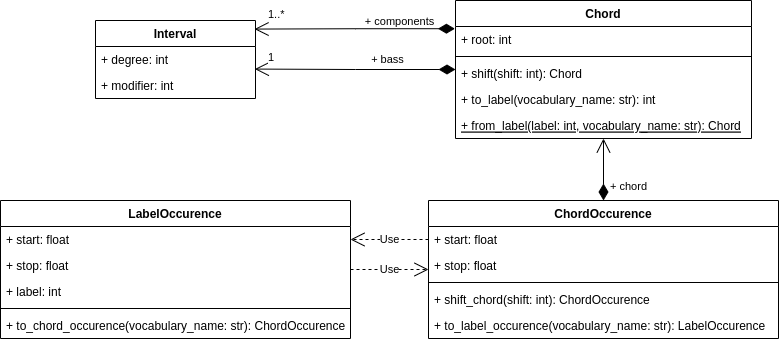
\includegraphics[width=1.0\textwidth]{./images/chord_model.png}
    \caption{Diagram klas UML przedstawiający model obiektowy akordów muzycznych.}
    \label{fig:chord_model}
\end{figure}

\subsection{Parsowanie plików \filetype{lab}}

% wstęp o formacie lab
Chris Harte w swojej pracy \cite{harte_towards_nodate}, zanim przedstawił szczegółowo autorski
format zapisu akordów, uzasadnił obszernie zapotrzebowanie na tego typu rozwiązanie i wyliczył
podstawowe idee, którymi się kierował. Wykazywał między innymi, że nie istnieje inny,
ustandaryzowany między gatunkami i szkołami, uniwersalny system zapisu akordów.  Wymieniał
podstawowe problemy z jakimi trzeba się mierzyć, poczynając od niejednoznaczności i ograniczeń
istniejących form zapisu, a kończąc na problemach związanych z dużym ryzykiem błędów w pisowni
niektórych symboli.

% opis słowny formatu lab
Zaproponowany przez niego format zapisu akordów odpowiada trzyczęściowej strukturze akordów.
Tekstowa reprezentacja akordu składa się kolejno z symbolu oznaczającego podstawę, listy interwałów
w postaci skrótu i/lub dodatkowych interwałów podanych jawnie oraz pojedynczego interwału na końcu
oznaczającego bas. Ogólna forma zapisu jest następująca: 
\begin{center}
    \code{root : shorthand (interval1, interval2...) / bass}
\end{center}
W przeciwieństwie do opisywanej wcześniej struktury danych, w przypadku zapisu tekstowego, podstawa
akordu zapisywana jest w postaci symbolicznej: nazwa jednego z 7 dźwięków (\code{ABCDEFG}), po której w
razie konieczności następują modyfikatory - krzyżyki i bemole, zapisywane odpowiednio jako znaki
\code{\#} oraz \code{b}. Następnie jest dwukropek, po którym zapisuje się listę interwałów. Może mieć ona
postać jawnej listy, poprzedzielanej przecinkami i ujętej w nawiasy, gdzie każdy interwał zapisywany
jest jako liczba całkowita oznaczająca stopień, w razie potrzeby poprzedzona krzyżykami lub
bemolami. Zamiast podawać listę można skorzystać z predefiniowanego skrótu, implikującego
odpowiednią listę interwałów. Przykładem takiego skrótu jest \code{min}, oznaczający ciąg interwałów
1, b3 i 5. Można również wykorzystać zarówno skrót jak i listę w nawiasach, dodając w ten
sposób dodatkowe interwały ponad te wynikające ze skrótu, lub usuwając wybrane interwały z
predefinowanej listy, poprzedzając je znakiem \code{*}. Niepodanie ani listy ani żadnego ze skrótów
traktuje się jako zwykły akord majorowy (interwały 1, 3 i 5). Na końcu występuje opcjonalny,
dodatkowy interwał oznaczający bas, poprzedzony znakiem \code{/}. Jeżeli bas nie jest podany, zakłada
się interwał prymy, czyli że podstawa akordu jest jednocześnieg jego najniższym dźwiękiem. Zapisany
według tej metody akord C-dur wygląda tak:
\begin{center}
    \code{C:(1,3,5)}
\end{center}
lub po prostu tak:
\begin{center}
    \code{C}
\end{center}
Z kolei akord Cis-moll w pierwszym przewrocie, bez użycia skrótu wygląda tak:
\begin{center}
    \code{C\#:(1,b3,5,b7)/b3}
\end{center}
Wykorzystując skóty, ten sam akord ma postać:
\begin{center}
    \code{C\#:min/b3}
\end{center}
Cały plik \filetype{lab} składa się z trzech kolumn oddzielonych białymi znakami (np. tabulatorami).
Pierwsza i druga kolumna zawierają liczby zmiennoprzecinkowe, oznaczające odpowiedni czas
rozpoczęcia i zakończenia trwania akordu w sekundach. Trzecia kolumna zawiera symbol akordu.

% parsowanie lark'iem - idea, gramatyka, transformer
Aby parsować pliki z oznaczeniami akordów wykorzystana została biblioteka
\emph{lark}\footnote{https://github.com/lark-parser/lark}. Biblioteka ta jest zestawem narzędzi,
pozwalającym generować parsery do języków bezkontekstowych ang. \emph{context-free
language}\footnote{https://en.wikipedia.org/wiki/Context-free\_language}. Język tego typu definiowany
jest przez odpowiednią gramatykę bezkontekstową ang. \emph{context-free
grammar}\footnote{https://en.wikipedia.org/wiki/Context-free\_grammar}, a przykładem takiego języka
jest praktycznie dowolny język programowania. Również format zapisu akordów stanowi przykład języka
bezkontekstowego i dlatego biblioteka \emph{lark} pozwala bardzo łatwo, w sposób wydajny i
uporządkowany parsować tego typu oznaczenia. Aby wygenerować instancję parsera, czyli obiektu
odpowiedzialnego za proces parsowania, trzeba przygotować opis gramatyki danego języka. Popularnym
sposobem opisywania gramatyki bezkontekstowej jest notacja Backusa-Naura (ang. \emph{Backus-Naur
form}, której wersję rozszerzoną (ang. \emph{Extended Backu-Naur
form})\footnote{https://en.wikipedia.org/wiki/Extended\_Backus-Naur\_form} wykorzystuje właśnie
biblioteka \emph{lark}. Tak więc przygotowany został plik
\url{src/annotation\_parser/labfile\_grammar.lark}, który zawiera definicję gramatyki formatu
\filetype{lab} (jego zawartość prezentowana jest w tabeli \ref{fig:lab_syntax}). Po sparsowaniu tekstu
według podanej gramatyki, parser tworzy drzewiastą strukturę, która dzieli ten tekst w sposób
hierarchiczny. Przechodząc przez tę strukturę wiadomo, jaką każdy fragment tekstu pełni logiczną
rolę (zgodnie z daną gramatyką) i jakiej większej konstrukcji jest on częścią. Biblioteka
\emph{lark} pozwala przygotować tzw. transformer, czyli obiekt który jest odpowiedzialny za
mapowanie ze wspomnianej struktury drzewiastej (wyniku parsowania) na własną, obiektową strukturę
danych. W pliku \url{src/annotation\_parser/labfile\_transformer.py} przygotowana została właśnie taka
klasa, która pozwala zamienić wynik parsowania pliku \filetype{lab} na instancje klas opisywanego
wcześniej modelu obiektowego, a dokładnie listę obiektów klasy \code{ChordOccurence}. Aby móc
przetłumaczyć tekstowe oznaczenia akordów na model obiektowy, potrzebne były mapowania z symboli
literowych reprezentujących dźwięki na wartości całkowite oraz ze skrótów na konkretne zbiory
interwałów. Mapy te w postaci słowników pythonowych zawiera plik
\url{src/annotation\_parser/labfile\_symbols.py}. Kod odpowiedzialny za stworzenie instancji
transformera i parsera oraz opakowanie tego w funkcję pomocniczą, umieszczony został w pliku
\url{src/annotation\_parser/\_\_init\_\_.py}. 

\begin{figure}
    \centering
    {\scriptsize \verbatiminput{../src/annotation_parser/labfile_grammar.lark}}
    \caption{Opis składni oznaczeń akordów \emph{lab} za pomocą rozszerzonej notacji Backusa-Naura.}
    \label{fig:lab_syntax}
\end{figure}

% tworzenie plików lab
Przygotowana została również możliwość wykonywania operacji odwrotnej do parsowania, czyli
wytwarzania plików \filetype{lab} z modelu obiektowego akordów, który z kolei może zostać wytworzony z
predykcji sieci. Nie została tutaj wykorzystana żadna specjalistyczna biblioteka - jedynie
podstawowe operacje na ciągach znaków, wraz ze wspomnianymi powyżej mapami symboli skrutów i symboli
dźwięków. Cała logika wytwarznia oznaczeń w formacie \filetype{lab} zawarta jest w plikuj
\url{src/annotation\_parser/labfile\_printer.py}.

\subsection{Parsowanie plików oznaczeń dla zbioru RS200}

% wstęp o formacie oznaczeń ze zbioru RS200
Format oznaczeń akordów wykorzystany w zbiorze RS200 jest znacznie mniej rozbudowany od formatu
\filetype{lab}. Jest to jednocześnie format znacznie mniej uniwersalny, nie rozwiązujący większości
problemów, które format \filetype{lab} rozwiązuje. Nawet dwóch badaczy, którzy równolegle przygotowywali
oznaczenia akordów dla zbioru RS200, aby później porównać je między sobą, tak naprawdę nie zachowali
spójnej konwencji, mimo iż razem stworzyli ten konkretny format zapisu. Z tego też powodu, jak już
wspomniane przy opisywaniu tego zbioru, dla ułatwienia zadania parsowania, wybrane zostały
oznaczenia tylko jednego z badaczy, który przygotował je w znacznie prostszy i bardziej
uporządkowany sposób.

% opis słowny formatu oznaczeń ze zbioru RS200
Każde wystąpienie akordu w utworze charakteryzowane jest przez rodzaj tego akordu i czas jego
wystąpienia. Jeżeli chodzi o to drugie, to autorzy zdecydowali się na wykorzystanie rekurencyjnej
składni (podobnej do notacji Backusa-Naura), wykorzystującej fakt, że utwory dzielą się na pewne
logiczne, powtarzalne części. Symbol każdego akord umieszczony jest w odpowiedniej części taktu, a
same takty są pogrupowane w większe struktury, które powtarzają się według określonych wzorców. W
ten sposób, za pomocą zaledwie kilku znaków, można opisać cały utwór. Jest to format jak najbardziej
czytelny dla człowieka, ale nie zawierający docelowej informacji, w której konkretnie sekundzie
zaczyna się i kończy dany akord. Na szczęście autorzy zbioru przygotowali również skrypty, które
łączą informacje o tempie utworu z oznaczeniami akordów. Skrypty te tworzą nowe pliki z oznaczeniami
(dostępne do pobrania i wykorzystane w tej pracy zamiast oryginalnych oznaczeń), które mają format
zbliżony do plików \filetype{lab}, gdzie pierwsza kolumna zawiera czas rozpoczęcia danego akordu. Jeżeli
chodzi o symbole akordów, to tutaj również autorzy poszli w kierunku relatywnego sposobu oznaczania,
ponieważ zamiast wykorzystać symbole konkretnych dźwięków, wykorzystują liczby rzymskie oznaczające
odległość względem toniki danego utworu.  Symbol każdego akordu składa się najpierw z liczby
rzymskiej, poprzedzonej ewentualnie modyfikatorem - krzyżykiem lub bemolem. Jeżeli znaki są małe, to
oznacza tryb minorowy, jeżeli wielkie, tryb majorowy. Następnie aż do znaku ukośnika mogą występować
dowolne symbole, informujące o modyfikacjach względem zwykłego trójdźwieku majorowego lub
minorowego. W praktyce są to informacje o występowaniu akordów septymowych, numerach przewrotów oraz
akordach, zwiększonych, zmniejszonych i występowaniu dodatkowych składników jak kwarta. Opcjonalnie,
na końcu może wystąpić znak ukośnika i kolejna liczba rzymska, oznaczająca akordy wtrącone (TODO
aplied chords). W praktyce symbol akordu wykorzystywany jest jedynie do stworzenia listy interwałów
i basu.  Podstawa akordu nie musi być wyliczana na podstawie liczby rzymskiej, ponieważ we
wspomnianym powyżej przetworzonym formacie oznaczeń, zawierającym kolumnę z czasem rozpoczęcia
akordu, dodane jest również kolumna z wartościami całkowitymi, reprezentującymi podstawę akordu
względem dźwięku C, a nie tonacji utworu.

% krótki opis implementacji, bo większość była opisana dla formatu lab
Jeżeli chodzi o parsowanie plików z oznaczeniami dla zbioru RS200, to również wykorzystana została
biblioteka \emph{lark}. Trzeba więc było przygotować odpowiedni opis gramatyki i odpowiednią klasę
transformującą na model obiektowy. To pierwsze znajduje się w pliku
\url{src/annotation\_parser/rs200\_dt\_grammar.lark} a to drugie w pliku
\url{src/annotation\_parser/rs200\_dt\_transformer.py}. Tabel \ref{fig:rs200_dt_syntax} prezentuje
zawartość pliku z gramatyką. Podobnie jak w przypadku parsowania formatu \filetype{lab}, plik
\url{src/anotation\_parser/\_\_init\_\_.py} zawiera kod tworzący instancję parser i transformera, oraz
opakowuje je w funkcję pomocniczą.

\begin{figure}
    \centering
    {\scriptsize \verbatiminput{../src/annotation_parser/rs200_dt_grammar.lark}}
    \caption{Opis składni oznaczeń akordów w zbiorze RS200 za pomocą rozszerzonej notacji Backusa-Naura.}
    \label{fig:rs200_dt_syntax}
\end{figure}


% skrypt evaluation, downloading, 02, 03 i 05 - znalezienie i pobranie najlepiej pasujących nagrań muzycznych
\section{Pozyskanie plików z nagraniami muzycznymi pasującymi do oznaczeń}

% to jest problem generalnie
Znalezienie odpowiednich plików z nagraniami muzycznymi stanowiło jeden z głównych problemów,
rozwiązywanych w ramach niniejszej pracy. Jest to problem z którym mierzyli się również twórcy
poprzednich rozwiązań, ponieważ tak jak wspomniano wcześniej, nieliczne zbiory oznaczeń
akordów dostarczane są zazwyczaj bez nagrań muzycznych, ze względu na prawa autorskie muzyków
(wyjątkiem jest oczyszczony z praw autorskich zbiór RWC POP).

% nie można tak po prostu łatwo ich wyszukać - opis i ocena ręcznej procedury
\subsection{Analiza koncepcji ręcznego wyszukiwanie nagrań} Pierwszym i prawdopodobnie
prowadzącym do najmniejszej liczby pomyłek sposobem pozyskania utworów muzycznych jest szukanie
,,ręczne''. Polegało by ono na znalezieniu odpowiednich artystów, albumów i konkretnych nagrań w
serwisach muzycznych oraz innych ogólnie dostępnych źródłach. W razie potrzeby wymagało by
zakupienie odpowiednich nagrań. Każdy zbiór oznaczeń należało by rozpatrzeć osobno i w miarę
możliwości spróbować pozyskać oryginalne, wykorzystane podczas tworzenia oznaczeń nagrania. W
przypadku zbioru RWC POP nagrania są możliwe do pozyskania za symboliczną opłatą. W przypadku
zbiorów Isohponics, Robbie Williams i uspop wiadomo, w miarę dokładnie, o które nagrania chodzi,
ponieważ dla każdego utworu znana jest nazwa albumu. Można próbować dostać się do tych konkretnych
albumów, weryfikując wyrywkowo, czy w znalezionych albumach oznaczenia pasują do nagrań. Możliwe
jest jednak, że trafi się na jakieś poprawione wydania, gdzie wszystkie utwory będą np. przesunięte
w czasie. Można wtedy próbować je ,,naprawić'' za pomocą odpowiedniego programu komputerowego. Co do
pozostałych zbiorów, to nie jest znany album i w tym przypadku zdecydowanie już nie można łatwo
stwierdzić, które spośród wielu możliwych nagrań będzie pasowało do oznaczeń. Trzeba by więc
samodzielnie odsłuchać fragment każdej znalezionej wersji nagrania i znaleźć tą odpowiednią, w
najgorszym przypadku odrzucając wszystkie i pozostając z samymi oznaczeniami akordów. Tak więc
metoda ta, chociaż najdokładniejsza, jest niezwykle czasochłonna i trudno skalowalna w przypadku
znalezienia większej liczby oznaczeń.  Co więcej i tak nie daje ona pewności, że nie trafią się
nagrania niepasujące, chyba że ostatecznie każde wybrane nagranie zostanie przesłuchane i porównane
z oznaczeniami akordów. Warto zaznaczyć, że cały opis powyższej procedury ,,ręcznej'', choć
przemyślany, jest jedynie teoretyczny (nie był zrealizowany od początku do końca) i nie wiadomo,
jakie problemy okazałyby się mało znaczące, a jakie nie zostały wzięte pod uwagę. 

% motywacja i decyzja o procedurze automatycznej
\subsection{Motywacja i decyzja o automatycznym wyszukiwaniu nagrań}
W ramach niniejszej pracy zdecydowano się na automatyczną procedurę wyszukiwania odpowiednich
utworów muzycznych w serwisie YouTube Music\footnote{music.youtube.com}. Takie podejście prowadzi
prawdopodobnie do pozyskania większej ilości niepasujących nagrań i co ważniejsze, w ogóle do
pozyskania mniejszej ilości nagrań. Jest to jednak podejście zdecydowanie szybsze. Automatyzacja
procesu wyszukiwania odpowiednich nagrań sama w sobie stanowi ciekawy problem, ktorego możliwe
rozwiązania wydają się być cenne, ze względu na swoją szybkość, powtarzalność i skalowalność.
Ponadto rozwiązuje częściowo problem reprodukcji i kontynuacji badań przez inne osoby.  Przygotowane
w ramach niniejszej pracy skrypty można by umieścić w internecie ułatwiając zadanie innym osobom
zajmującym się tym samym tematem. Nie można natomiast rozpowszechniać w ten sposób nagrań
muzycznych. Z tych powodów zdecydowano się, że ostatecznie zbiór danych oznaczonych będzie
prawdopodobnie trochę mniejszy i bardziej zanieczyszczony, niż w przypadku ręcznego wyszukiwania
odpowiednich utworów. Poświęcono natomiast czas na przygotowanie nieskomplikowango algorytmu,
opierającego się na kilku prostych założeniach, pozwalającego automatycznie wyszukiwać odpowiednie
nagrania w serwisie YouTube Music. Algorytm ten można opisać w kilku prostych krokach. Wśród nich
występują jednak trzy bardziej złożone operację: wyszukiwanie utworu w serwisie YouTube Music,
pobieranie konkretnego nagrania na dysk lokalny oraz ewaluacja tego nagrania - oceny na ile jest ono
zgodne z dostępnymi oznaczeniami akordów. Wszystkie trzy operacje są szczegółowo opisane poniżej.

% opis wyszukiwania utworów i liba ytmusicapi
\subsection{Wyszukiwanie utworów w serwisie YouTube Music}
Wyszukiwanie utworów w serwisie YouTube Music zostało wykonane za pomocą nieoficjalnego klienta
pythonowego do tego serwisu - \emph{ytmusicapi}\footnote{https://github.com/sigma67/ytmusicapi}.
Daje on mniej więcej takie same możliwości jak korzystanie z oficjalnego, graficznego klienta
przeglądarkowego. Można jednak wszystkie operacje łatwo zautomatyzować. Jest to przykład tak zwanego
\emph{web scrappingu}, który w tym przypadku jest niezbędny, jako że oficjalne API do tego (pod)serwisu
nie istnieje, a dostępne w ograniczonym zakresie (ograniczona liczba zapytań) API do całego serwisu
YouTube nie daje wystarczających możliwości przeszukiwania dostępnych tam nagrań muzycznych.
Korzystanie z klienta \emph{ytmusicapi} jest niezwykle proste. Trzeba jedynie stworzyć
instancję obiektu \code{YTMusic} (jest to dostęp analogiczny jak dla niezalogawnego użytkownika w
przeglądarce) i wywołać metodę \code{search} przyjmującą tekstowe zapytanie (takie jak wpisywane w
pole wyszukiwania w kliencie graficznym) oraz filtr, ograniczający wyniki do danego typu treści, np.
tylko do nagrań muzycznych, lub tylko do filmów. W zwróconych wynikach dostępne są informacje o
indentyfikatorze zasobu (\code{video\_id}), tytule utworu, artyście (lub artystach) i albumie
(jeżeli dotyczy).

% opis pobierania utworów - skryptu i liba pytube
\subsection{Pobieranie nagrań z serwisu YouTube na dysk lokalny}
Pobieranie nagrań na dysk lokalny również jest zrealizowane za pomocą nieoficjalnego, pythonowego
klienta, tym razem już do całego serwisu YouTube -
\emph{pytube}\footnote{https://github.com/pytube/pytube}. Służy on właściwie nie tyle do
przeszukiwania serwisu YouTube co do pobieranie z niego całych filmów lub samych ścieżek dźwiękowych
w dostępnych formatach i jakościach. Aby z niego skorzystać trzeba stworzyć instancję klasy
\code{YouTube} podając jako argument adres URL konkretnego filmu, przy czym wystarczy oczywiście
znać jedynie jego \code{video\_id} (\url{http://youtube.com/watch?v=\emph{video\_id}}). Następnie
można filtrować dostępne formaty i ostatecznie pobrać wybrany strumień na dysk. Przygotowana została
funkcja pomocnicza (\url{src/dataset\_scripts/downloading.py}), która dla danego \code{video\_id},
jeżeli nagranie nie zostało już pobrane (nie istnieje plik we wskazanym katalogu), wybiera pośród
dostępnych strumieni z samym dźwiękiem ten w najlepszej jakości i zapisuje go jako plik dźwiękowy do
wskazego katalogu. Pobieranie to może się z różnych powodów nie powieść (błąd sieci, YouTube odrzuca
podejrzane żądanie, etc.).

% opis idei ewaluacji nagrań i liba madmom
\subsection{Ewaluacja nagrań - ocena dopasowania do oznaczeń akordów}
Ewaluacja nagrań jest najbardziej skomplikowaną i jednocześnie najważniejszą częścią całego procesu
wyszukiwania nagrań. Aby automatycznie ocenić czy nagranie pasuje do oznaczeń trzeba automatycznie
rozpoznać jakie akordy w nim występują. Z kolei przygotowanie algorytmu rozpoznającego akordy
stanowi jeden z podstawowych celów niniejszej pracy. Oczywiście nie można się więc na tym etapie
posłużyć własnym rozwiązaniem. Istnieje natomiast dużo gotowych, wysokopoziomowych bibliotek, które
realizują to zadanie, z większą bądź mniejszą dokładnością. Wysoka dokładność takiego algorytmu nie
ma na tym etapie dużego znaczenia, chodzi jedynie aby poglądowo ocenić, czy dane nagranie pasuje do
oznaczeń, czy może jest to zupełnie inny utwór, czy jedynie inna, wolniejsza lub trochę przesunięta
w czasie wersja oryginalnego nagrania. Zdecydowano się na użycie biblioteki
\emph{madmom}\footnote{https://github.com/CPJKU/madmom}, której autorem jest sam Korzeniowski.
Biblioteka ta, podobnie jak dwie poprzednie i w ogóle zdecydowana większość bibliotek języka Python,
jest bardzo prosta w użyciu. Trzeba wybrać odpowiedni algorytm, stworzyć jego instancję i wywołać
przekazując ścieżkę do pliku. Pod spodem wykorzystywana jest biblioteka \emph{ffmpeg} do odczytania
praktycznie dowolnego formatu. Za pomocą wytrenowanego wcześniej modelu rozpoznawane są występujące
akordy (standardowe 25 klas) i zwracane są czasy ich występowania oraz symbole w formacie
wykorzystywanym w plikach \filetype{lab} (zgodnym z \cite{harte_towards_nodate}). Ze względu na
niewielkie wymagania dotyczące jakości klasyfikacji i większe wymagania dotyczące szybkości
działania, zdecydowano się użyć prostszego z dwóch dostępnych algorytmów, czyli \emph{Deep Chroma
Extractor} \cite{korzeniowski_feature_2016}.

% dokładny opis procedury ewaluacji (skryptu ewaluacyjnego)
Cała procedura ewaluacji nie kończy się na wywołaniu biblioteki i rozpoznaniu występujących akordów.
Trzeba wybrać odpowiednie metryki pozwalające łatwo porównać między sobą kilka dostępnych nagrań dla
tego samego zestawu oznaczeń akordów. Po pierwsze wykorzystana została podstawowa miara WCSR. Po drugie
dla każdego nagrania liczone jest przesunięcie czasowe pomiędzy początkiem pierwszego oczekiwanego
(z pliku z oznaczeniami) i pierwszego rozpoznanego (za pomocą biblioteki madmom) akordu
(\code{start\_diff}), oraz przesunięcie czasowe pomiędzy końcem ostatniego oczekiwanego i ostatniego
rozpoznanego akordu (\code{stop\_diff}). Oczywiście poprzez wystąpienie akordu rozumie się
wystąpienie akordu dowolnej klasy poza \emph{no chord}. Realizująca wszystkie te operacje funkcja
pomocnicza znajduje się w pliku \url{src/dataset\_scripts/evaluation.py}. W przypadku, gdy żaden akord
nie występuje w oznaczeniach lub nie został rozpoznany, funkcja ta nie zwraca żadnych wartości.

% interpretacja metryk
Metryka WCSR pozwala ocenić na ile znalezione akordy są zgodne z oczekiwanymi. Metryki prezentujące
przesunięcie czasowe dodatkowo pozwalają wykryć sytuację, kiedy znalezione nagranie zaczyna się w
innym momencie albo jest zdecydowanie za długie. W obu tych sytuacjach wciąż możliwa jest względnie
wysoka wartość miary CSR. W konsekwencji miara ta nie pozwala łatwo wyeliminować nagrań, ktore z
powodu różnej długości z całą pewnością nie pasują do oznaczeń.

% opis całego algorytmu ze skryptu 02
\subsection{Algorytm automatycznego wyszukiwania pasujących nagrań muzycznych}
Poniższe kroki są wykonywane dla każdej pozycji z indeksu (\url{data/index.csv}) opisującego cały
dostępny zbiór oznaczeń. Przechodzenie przez cały indeks dzieje się równolegle w 16 procesach, jako
że w zastosowanym algorytmie nie ma żadnych zależności między poszczególnymi utworami. Wynikiem
działania algorytmu są dodatkowe kolumny w pliku \url{index.csv}, prezentujące identyfikator
najlepszego znalezionego nagrania (\code{video\_id}) oraz wyniki ewaluacji tego nagrania:
przesunięcie początku pierwszego akordu (\code{start\_diff}) i zakończenia ostatniego
(\code{stop\_diff}) względem pliku z oznaczeniami oraz wartość miary CSR (\code{csr}).

Poniższy algorytm jest dodatkowo przygotowany w taki sposób, aby móc wykonywać go wielokrotnie dla
tego samego indeksu w celu wyszukiwania nagrań dla nowo dodanych plików z oznaczeniami, skorzystania
z dostępnych od niedawna nagrań lub po prostu kontynuacji przerwanego działania, które jest
czasochłonne i może zostać przerwane z powodu różnych błędów.

Kroki algorytmu są następujące:
\begin{enumerate}
    \item Jeżeli dany utwór ma już dopasowane nagranie (\code{video\_id}) i jest ono zewaluowane to
        zakończ działanie.
    \item Jeżeli dany utwór ma już dopasowane \code{video\_id} i NIE jest ono zewaluowane to zrób
        ewaluację tego nagrania i zakończ działanie.
    \item Wyszukaj nagrania w serwisie YouTube Music zapytaniem ,,tytuł artysta album (jeśli jest
        znany)'', filtr ustawiony na nagrania muzyczne, ogranicz do 10. wyników.
    \item Pierwszy etap selekcji - na podstawie nazw. Etap ten ma na celu zmniejszyć liczbę
        czasochłonnych ewaluacji z etapu drugiego. 
        \begin{enumerate}
            \item Znormalizuj nazwy albumu, utworu i artystów dla danego utworu i we wszystkich
                wynikach wyszukiwania poprzez zamianę wielkich liter na małe i pozostawienie tylko
                znaków alfanumerycznych oraz znaku ,,\_''
            \item Wybierz te wyniki wyszukiwania, dla których nazwy albumu (jeśli jest
                dostępna), utworu i artystów zawierają w sobie odpowiednie nazwy z indeksu.
            \item Jeżeli żadne nagranie nie pasuje na tym etapie, wszystkie przechodzą dalej.
        \end{enumerate}
    \item Drugi etap selekcji - na podstawie ewaluacji.
        \begin{enumerate}
            \item Pobierz na dysk nagrania z pozostałych po etapie pierwszym wyników wyszukiwania
            \item Dokonaj ewaluacji każdego z pobranych nagrań i zapamiętaj wartości metryk
            \item Usuń nagrania z dysku
            \item Wybierz to nagranie, które ma najwyższą wartość WCSR i zapisz w indeksie jego
                \code{video\_id} oraz wartości metryk z ewaluacji
        \end{enumerate}
\end{enumerate}

% opis skryptu 03 - selekcja i podział na trening/test/walidacja
\subsection{Selekcja i podział utworów, dla których znaleziono dobre nagranie}
Na tym etapie indeks opisujący wszystkie dostępne pliki z oznaczeniami był rozszerzony o kolumny
zawierające informacje o identyfikatorze nagrania z YouTube oraz o metrykach z ewaluacji tego
nagrania. Chociaż prawie dla każdego pliku z oznaczeniami znalezione zostało jakieś
\code{video\_id}, to w wielu przypadkach nagranie to zupełnie nie pasowało do oznaczeń. Trzeba było
ustalić pewną granicę decyzyjną, opartą o wartości metryk, według której nagrania zostaną uznane za
pasujące do plików z oznaczeniami. Znalezienie takiej granicy nie było trywialne. Należało wybrać
losowo niewielką część nagrań ze zróżnicowanymi wynikami ewaluacji, odsłuchać fragmenty tych nagrań
i ocenić, co w praktyce oznaczają takie a nie inne wartości metryk. Głównie chodziło o to, aby
stwierdzić, jakie są możliwe przyczyny słabych wyników ewaluacji, z czego wynikają przesunięcia w
początku i zakończeniu utworu oraz czy zawsze implikują one niepasujące nagranie. Praca ta była
chaotyczna i nie została udokumentowana w żaden specjalny sposób. Jedynym jej wynikiem jest
zdecydowanie się na wykorzystanie jedynie tych nagrań, dla których wartość CSR była większa niż
0.3, a wartość bezwzględna przesunięcia końca utworu mniejsza niż 10 sekund. Warunek ten prezentuje
poniższe równanie:
\begin{center}
    \code{CSR > 0.3 AND |stop\_diff| < 10}
\end{center}
Oczywiście granica ta jest bardzo umowna - nie ma żadnej pewności, że wśród wykorzystanych nagrań
nie ma nagrań błędnych, jak i że wśród nagrań usuniętych, nie ma nagrań poprawnych. Nie udało się
niestety znaleźć innej metody ewaulacji i ostatecznie trzeba było zdecydować się na jakąś wartość
progową, wiedząc, że opiera się ona po części na intuicji, a po części na ślepym losie.

Operację odfiltrowania ,,niepasujących'' nagrań zaimplementowano w skrypcie
\url{src/dataset\_scripts/03-select\_proposals\_and\_split.py}. Po wykonaniu progowania z 1268 utworów
pozostało jedynie 995. Następnie usuwane są również te utwory, które mają dopasowane to samo
nagranie co inny utwór. Znalazł się tylko 1 taki przypadek. Tak więc ostatecznie pozyskano nagrania
dla 994 utworów. W ramach tego samego skryptu, wszystkie te utwory zostały podzielone na 3
podzbiory: treningowy, testowy i walidacyjny w proporcjach odpowiednio $8:1:1$ (ramach każdego
zbioru oznaczeń). Podział ten został zapisany w nowej kolumnie \code{purpose} w pliku
\url{data/index.csv}. Wpis w tej kolumnie jest jednocześnie znacznikiem, że dla danego pliku z
oznaczeniami znaleziono pasujące nagranie.

\subsection{Pobieranie utworów i podsumowanie ich liczebności}

Ostatnim etapem jest ponowne pobranie wszystkich nagrań z serwisu YouTube. Operacja ta została
wydzielona do osobnego kroku i osobnego skryptu, ponieważ nagrania te zajmują względnie dużo miejsca
i dodatkowo nie powinny być rozpowszechniane. Dzięki temu nie muszą być więc przechowywane a mogą
być z łatwością od nowa pobrane z serwisu YouTube, kiedy projekt jest klonowany lub przenoszony na
inną maszynę. Mając więc gotowy plik indeksu, stanowiący stałą część repozytorium projektu, należy
wywołać skrypt \url{src/dataset\_scripts/05-download\_songs.py}, który pobiera wszystkie nagrania z
pliku indeksu, dla których istnieje wartość w kolumnie \code{purpose}. Pobiera je, wykorzystując
opisaną wcześniej funkcje pomocniczą z pliku \url{src/dataset\_scripts/downloading.py}, czyli
wybierając najlepszy dostępny strumień dźwiękowy i zapisując go w postaci pliku dźwiękowego, w
katalogu \url{data/audio}. Dodatkowo do pliku indeksu dodawana jest nowa kolumna
\code{audio\_filepath}, która dla każdego pobranego utworu zapisuje ścieżkę do pliku dźwiękowego.

Tabela \ref{tab:datasets2} prezentuje rozkład 994 pobranych i wykorzystywanych do eksperymentów
nagrań, pomiędzy poszczególne zbiory danych z oznaczeniami. Tabela \ref{tab:datasets3} prezentuje
natomiast liczebność nagrań w zbiorach treningowym, testowym i walidacyjnym. Nagrania pobierane są w
najlepszej dostępnej jakości. Prawie wszystkie pliki (z wyjątkiem dwóch) zostały pobrane w formacie
\filetype(webm), z częstotliwością próbkowania $48000$Hz i $32$-bitową dokładnością zapisu.
Pozostałe dwa nagrania pobrane zostały w formacie \filetype(mp4) z częstotliwością próbkowania
$44100$ i tą samą dokładnością zapisu.

Jak widać w tabeli \ref{tab:datasets2}, nie udało się znaleźć żadnego pasującego nagrania do
oznaczeń ze zbioru RWC POP. Jest to spowodowane faktem, że większość utworów w tym zbiorze to
japońska muzyka popularna, która nie jest dostępna, lub nie udało się jej wyszukać zastosowaną
metodą w serwisie YouTube Music. Sytuacja ta jest jednak zupełnie akceptowalna i zrozumiała w
kontekście próby stworzenia całkowicie automatycznego algorytmu wyszukiwania odpowiednich nagrań w
Internecie.

\begin{table}
    \centering
    \caption{Liczebności pobranych i wykorzystywanych do eksperymentów nagrań między poszczególnymi zbiorami danych z oznaczeniami.}
    \label{tab:datasets2}
    \begin{tabular}{|l|c|c|}
        \hline
        Nazwa zbioru & Liczba nagrań & Łączny czas trwania [h] \\
        \hline
        Isophonics          & $217$ & $10.5$ \\ % Loaded 217 songs (10:18:27)
        McGill Billboard    & $420$ & $24.5$ \\ % Loaded 420 songs (1 day, 0:34:52)
        Robbie Williams     & $54$  & $4$    \\ % Loaded 54 songs  (4:10:22)
        RS200               & $142$ & $8.5$  \\ % Loaded 142 songs (8:43:31)
        RWC POP             & $0$   & $0$    \\
        Uspop2002           & $161$ & $11.5$ \\ % Loaded 161 songs (11:19:29)
        \hline
        SUMA                & $994$ & $59$   \\
        \hline
    \end{tabular}
\end{table}

\begin{table}
    \centering
    \caption{Liczności zbiorów treningowego, testowego i walidacyjnego.}
    \label{tab:datasets3}
    \begin{tabular}{|l|c|c|}
        \hline
        Nazwa zbioru & Liczba nagrań \\
        \hline
        Treningowy  & 790 \\
        Testowy     & 102 \\
        Walidacyjny & 102 \\
        \hline
    \end{tabular}
\end{table}

Mając już wybrane, które konkretnie utwory będą wykorzystywane do eksperymentów, można było zbadać
rozkład częstości występowania poszczególnych typów akordów w tych utworach. Rysunek
\ref{fig:chords_histogram} prezentuje ile godzin zajął sumarycznie każdy z $25$ rozpoznawanych typów
akordów.

\begin{figure}
    \centering
    \makebox[\textwidth][c]{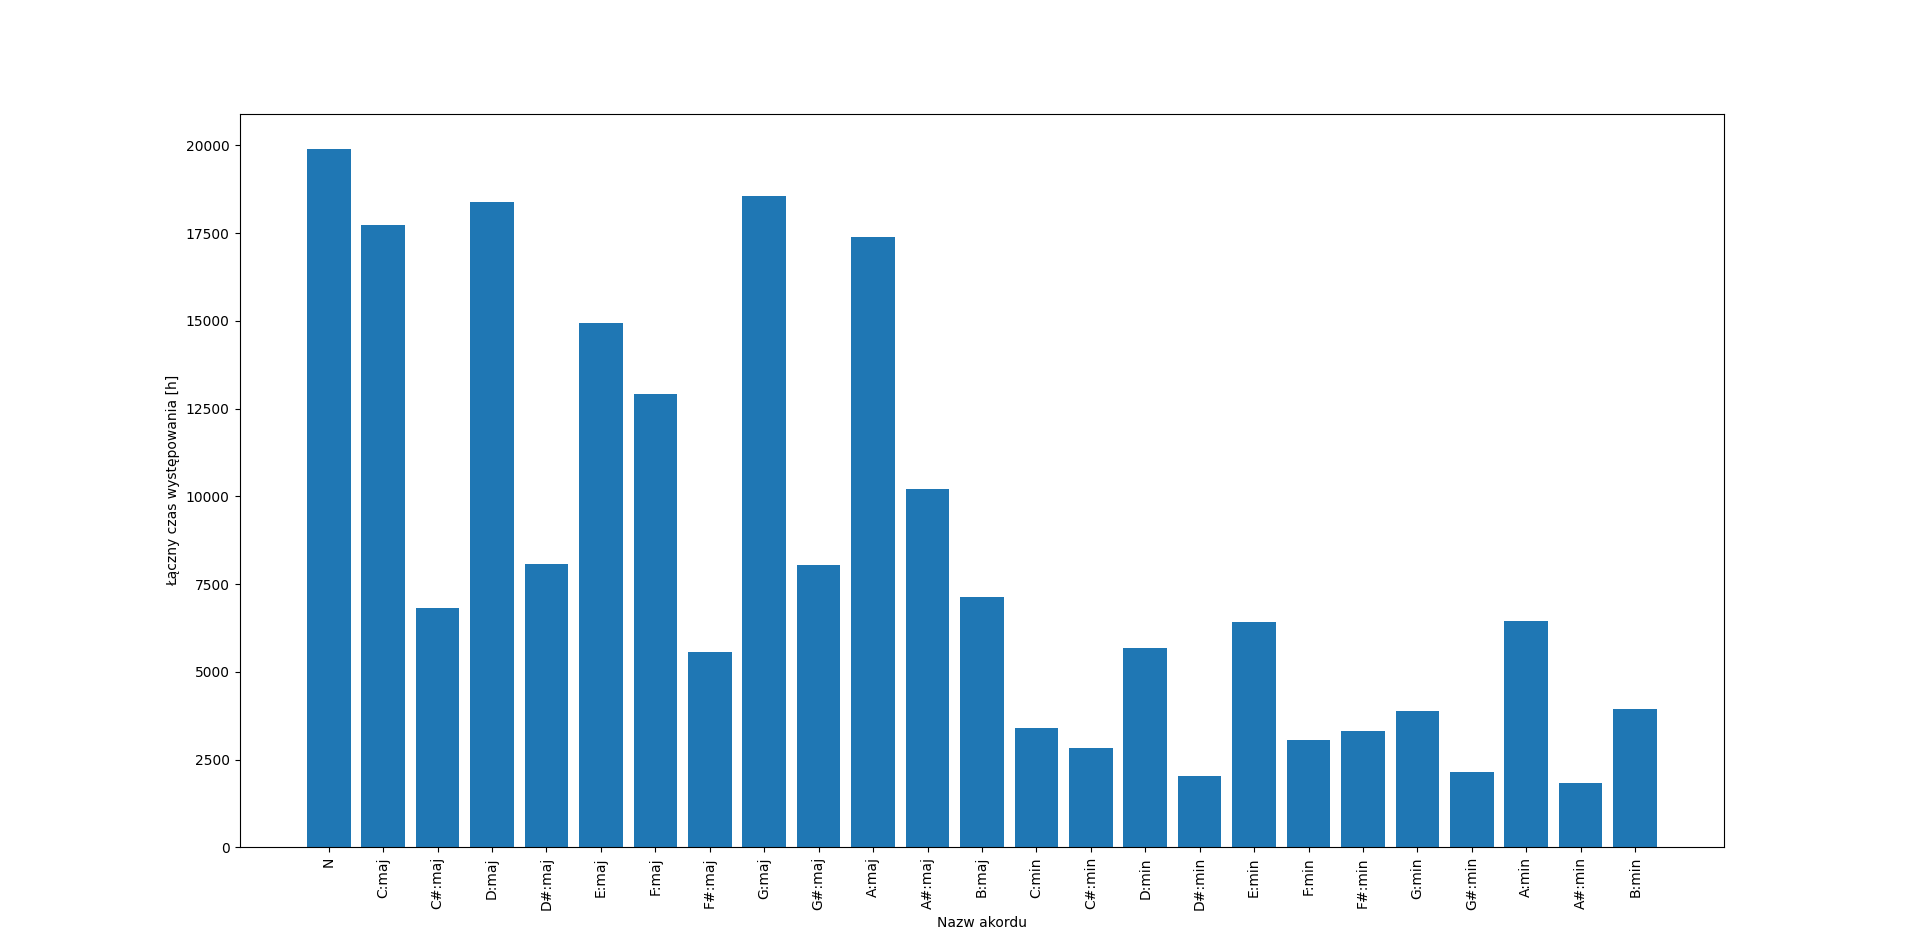
\includegraphics[width=1.7\textwidth]{./images/chords_histogram.png}}
    \caption{Rozkład występowania każdej z $25$ klas akordów w $994$ utworach wykorzystywanych w eksperymentach}
    \label{fig:chords_histogram}
\end{figure}


\section{Wyszukiwanie utworów bez oznaczeń z rankingów magazynu Billboard}

% TODO: statystyki o zbiorze nieoznaczonym
% wstęp
Jak już wspomniano wcześniej, zgromadzenie zbioru danych nieoznaczonych było znacznie prostsze. Dla
przypomnienia, chodzi tutaj jedynie o same nagrania muzyczne, bez oznaczeń akordów. W najprostszym
rozumieniu wystarczyło by więc pobrać dowolną liczbę dowolnych nagrań muzycznych z internetu i
zadanie będzie wykonane. Trzeba natomiast zorganizować ten proces w taki sposób, aby nagrania te
się nie powtarzały i aby, co ważniejsze, stanowiły pewną reprezentatywną próbę dla muzyki danego
gatunku, w tym przypadku dla popularnej muzyki zachodniej (ang. \emph{Western Music}). Trzeba więc
uniknąć sytuacji, kiedy zbyt wiele nagrań będzie pochodziło z tego samego okresu, z tego samego
specyficznego nurtu, lub nawet od tego samego artysty. W ramach niniejszej pracy zdecydowano się na
bardzo proste podejście do tematu wyboru tychże utworów - były one losowo próbkowane (bez powtórzeń)
ze wszystkich dostępnych rankingów \emph{Hot 100} magazynu \emph{Billboard}. Jest to więc metoda
niejako skopiowana od twórców zbioru McGill Billobard. Zapewnia ona, że wybrane utwory będą z
różnych okresów, od różnych artystów i w różnych stylach. Będą również, ze względu na swoją wysoką
popularność, stanowiły reprezentatywną grupę muzyki popularnej zachodu. Znalezione w ten sposób
utwory były następnie wyszukiwane w serwisie YouTube Music i w razie dostępności pobierane i
dodawane do pliku indeksu. Wyszukanych i pobranych tą metodą zostało 10000 różnych nagrań.

Cały alogorytm automatycznego preszukiwania rankingów magazynu \emph{Billboard} oraz serwisu YouTube
Music został zaimplementowany w skrypcie \url{src/dataset\_scripts/04-collect\_big\_dataset.py}. Jest
to implementacja umożliwiająca przeszukiwanie w wielu wątkach jednocześnie (w ramach pracy
wykorzystanych zostało 5 wątków), ze względu na to, że krytycznymi pod wzlędem czasu operacjami są
zapytania do Internetu, a cała procedura jest czasochłonna. Algorytm ten składa się z dwóch
zasadniczych części: pierwsza związana jest z przeszukiwaniem rankingów \emph{Hot 100} a druga z
wyszukiwaniem kandydujących utworów w serwisie YouTube Music.

Pierwsza z dwóch części algorytmu została zaimplementowana w postaci pythonowego generatora o nazwie
\code{billboard\_hot100\_item\_generator}. Generator ten zaczyna od stworzenia listy dat wszystkich
niedziel od 9 kwietnia 1958 roku, z kiedy to dostępny jest najstarszy, cotygodniowy ranking
\emph{Hot 100} magazynu \emph{Billboard}. Ranking ten prezentuje najpopularniejsze w danym tygodniu
utwory z różnych gatunków muzycznych, mierzone według aktywności serwisów streamingowych. Każda data
z powstałej listy odpowiada zatem jednemu rankingowi, ze wszystkich dostępnych, od najstarszego aż
do teraz. Zwracając kolejne wyniki, generator iteruje przez te wszystkie daty w losowej kolejności.
Dla każdej z nich wykonuje zapytanie do serwisu internetowego magazynu
\emph{Billboard}\footnote{https://www.billboard.com/charts}, wykorzystując w tym celu dedykowaną
pythonową bibliotekę \emph{billboard.py}\footnote{https://github.com/guoguo12/billboard-charts}.
Zapytanie to zwraca dla danej daty listę tytułów utworów, wraz z nazwiskami artystów (album nie jest
znany). Przechodząc przez kolejne rankingi generator zapisuje i sprawdza, czy znalezione utwory nie
były już wcześniej zwrócone, ponieważ często się zdarza, że ten sam utwór występuje na wielu
rankingach. Podsumowując, generator ten dostarcza losowe pozycje z rankingów \emph{Hot 100} magazynu
\emph{Billboard} w postaci jednej, bardzo długiej, niezawierającej powtórzeń, generowanej
dynamicznie listy.

Drugą część implementacji stanowi uruchamiana w wielu wątkach jednocześnie funkcja
\code{find\_next\_hot\_song}. Zadaniem tej funkcji jest pobrać kolejną parę tytuł-nazwisko z
opisywanego powyżej generatora i wyszukać ją w serwisie YouTube Music. Wyszukiwanie przebiega z
pomocą opisywanej wcześniej biblioteki \emph{ytmusicapi}. Wyniki wyszukiwania są ograniczone do
utworów muzycznych. Spośród pierwszych trzech wyników brany jest pierwszy taki, którego
\code{video\_id} nie zostało już pobrane dla jakiegoś innego utworu. Jeżeli znajdzie się takie
nagranie, to jest ono pobierane na dysk (za pomocą opisywanego wcześniej skryptu pomocniczego z
pliku i biblioteki \emph{pytube}) i dodawane do pliku indeksu. Wszystkie znalezione w ten sposób
nagrania mają specjalną wartość \code{,,pretrain''} w kolumnie \code{purpose}. Oczywiście wiersze
indeksu związane z tymi nagraniami nie mają zapisanej ścieżki do pliku z oznaczeniami.

W przypadku wyszukiwania dużej liczby utworów za pomocą tego algorytmu może dojść do sytuacji, że
znalezione nagrania będą się powtarzać, nie będą związane z danym utworem lub, że w ogóle nie uda
się znaleźć nagrania dla danego zapytania. Wszystkie te przypadki zostały rozważone i ze względu na
naturę tego wyszukiwania nie są problematyczne. Algorytm został napisany tak, aby wszystkie wyniki
były unikalne. Jeżeli nie uda się znaleźć unikalnego nagrania, po prostu algorytm przechodzi do
kolejnej, losowej pozycji z rankingów \emph{Billboard}, aż nie zwróci zadanej liczby różnych nagrań
z serwisu YouTube Music. Nagrania niepasujące do wyszukiwanych tytułów utworów również nie
są problematyczne, ponieważ wykorzystanie tutaj tych a nie innych tytułów jest jedynie pewnym
punktem wyjścia do zgromadzenia dużej liczby różnorodnych, popularnych nagrań. Pojedyncze przypadki
nagrań spoza tej konkretnej listy nie stanowią najmniejszego problemu, są nawet pożądane, ze względu
na różnorodność zbioru.

\section{Wstępne przetwarzanie danych}

% TODO: dodać jakiś ładny schemat prezentujący cały preprocessing (obrazki spektrogramów itd.)
% wstęp
W poprzednich podrozdziałach opisany został proces zgromadzenia plików z oznaczeniami, zgromadzenia
plików z nagraniami i utworzenia indeksu, opisującego cały powstały zbiór danych. Ostatnim etapem
prac, związanym z przygotowaniem danych, jest przedstawienie ich w formie nadającej się na wejście
sieci neuronowej. Całe to \emph{wstępne przetwarzanie danych} (ang. \emph{preprocessing}) zostało
przygotowane na podstawie \cite{park_bi-directional_2019}, ponieważ to właśnie ta praca stanowi
główny punkt odniesienia dla otrzymanych wyników. Wszystkie opisane poniżej kroki przetwarzania
zgromadzonych danych, zostały zaimplementowane w postaci pytorchowej klasy \code{Dataset}, w pliku
\url{src/training/dataset.py}.

\subsection{Wstępne przetwarzanie plików dźwiękowych}

\subsubsection{Wczytywanie plików}

% format zapisu dźwięku
W swojej surowej, nieskompresowanej postaci, plik dźwiękowy ma postać długiego ciągu, lub kilku
ciągów próbek. Każdy taki ciąg (tzw. kanał), reprezentuje inną część nagrania (np. inny instrument,
inne źródło nagrywania). Próbki z kolei są po prostu liczbami rzeczywistymi, reprezentującymi w
sposób dyskretny falę dźwiękową (jej stan w kolejnych chwilach czasu). Taka cyfrowa reprezentacja
sygnału dźwiękowego pozwala odtworzyć nagranie za pomocą odpowiedniego sprzętu lub wykonać
najróżniejsze analizy, w tym również rozpoznawanie akordów.

% wczytywanie surowych danych
Aby wczytać zapisane na dysku pliki dźwiękoweo do programu pythonowego w opisanym powyżej, surowym
formacie, wykorzystana została popularna biblioteka \emph{librosa} \cite{mcfee_librosa_2015}. Ma ona
bardzo prosty i przejrzysty interfejs. Między innymi dostarcza funkcję \code{load}, która przyjmuje
ścieżkę do pliku i zestaw parametrów, na podstawie których wczytuje nagranie z dysku, resampluje
jeśli trzeba i zwraca w formie tablicy próbek. Wykorzystane parametry ładowania nagrań za pomocą tej
funkcji zostały wymienione w tabeli \ref{tab:load_audio_params}. Generalnie podczas ładowania,
niezależnie od formatu pobranych z serwisu YouTube plików wejściowych, wszystkie nagrania są
resamplowane do częstotliwości $22050$Hz a wszystkie kanały są miksowane do jednego.

\begin{table}
    \centering
    \caption{Parametry ładowania nagrań muzycznych za pomocą bibiloteki \emph{librosa}}
    \label{tab:load_audio_params}
    \begin{tabular}{|l|l|} \hline
        Docelowa liczba kanałów & 1 \\ \hline
        Docelowa częstotliwość próbkowania & 22050Hz \\ \hline
        Algorytm resamplingu & \code{kaiser\_fast} \\ \hline
    \end{tabular}
\end{table}

\subsubsection{Tworzenie spektrogramów}

% uzasadnienie wykorzystania spektrogramów
Istnieją modele, dla których gotowym formatem wejściowym jest jedynie zresamplowany do odpowiedniej
częstotliwości surowy sygnał dźwiękowy \cite{baevski_wav2vec_2020}. Jednakże, w zadaniu
rozpoznawania akordów, praktycznie zawsze stosuje się dodatkowy etap wstępnego przetwarzania sygnału
dźwiękowego: przejście w dziedzinę czestotliwości, czyli stworzenie spektrogramu. Może mieć on różne
formy, ale zazwyczaj bazuje na dyskretnej transformacji Fouriera, lub powiązanej z nią dyskretnej
transformacji kosinusowej. Ta dwuwymiarowa reprezentacja dźwięku była szczególnie korzystna w
przypadku klasycznych metod rozpoznawania akordów. Spowodowane jest to tym, że bezpośrednio zawiera
informacje o wysokościach poszczególnych dźwięków składowych, jest więc łatwa w interpretacji i
czytelna dla człowieka. W przypadku modeli jakimi są sieci neuronowe, reprezentacja ta nie jest już
tak krytyczna, sieć może bowiem względnie łatwo sama nauczyć się najlepszej transformacji dla danego
zadania. Ponieważ jednak spektrogramy są wciąż powszechnie wykorzystywane w obszarze MIR, w ramach
tej pracy również wykorzystana została ta reprezentacja. 

% metoda i parametry tworzenia spektrogramów
Do utworzenia spektrogramów również została wykorzystana biblioteka \emph{librosa}, a dokładnie
funkcja \code{cqt}. Jak wynika z nazwy tej funkcji, w ramach niniejszej pracy utwory były
prezentowane za pomocą spektrogramów na bazie transformacji kosinusowej. Ponieważ wynik tej
transformacji ma postać zespoloną, z surowych spektrogramów wyliczana jest wartość bezwzględna,
która jest jeszcze dodatkowo logarytmowana. Szczegółowe wartości parametrów wykorzystanych do
stworzenia spektrogramów prezentowane są w tabeli \ref{tab:spectrogram_params}. Nagrania jest więc
dzielone na ramki, z częstotliwością około $11$ ramek na sekundę. Każda z nich reprezentowana jest
przez wektor $144$ wartości, które informują o natężeniu poszczególnych dźwięków (w skali
logarytmicznej) w danej chwili czasu. Na samym końcu wartości spektrogramów są jeszcze globalnie
standaryzowane --- odejmuje się od nich średnią wartość całego zbioru i dzieli przez odchylenie
standardowe.

\begin{table}
    \centering
    \caption{Parametry tworzenia spektrogramów za pomocą biblioteki \emph{librosa}}
    \label{tab:spectrogram_params}
    \begin{tabular}{|l|l|} \hline
        Rozmiar ramki & $2048$ (około $0.09$s) \\ \hline
        Częstotliwość minimalna & $32.703$Hz (dźwięk \code{C1}) \\ \hline
        Liczba składowych & $144$ ($6$ oktaw) \\ \hline
        Liczba składowych na oktawę & $24$ ($2$ na półton) \\ \hline
    \end{tabular}
\end{table}

% implementacja
Chociaż do eksperymentów wykorzystane zostały jedynie opisane powyżej spektrogramy CQT, program
został przygotowany w sposób umożliwiający inną metodę przetwarzania wstępnego. Jedyne założenie
jest takie, że ciąg próbek wejściowych dzielony jest na ramki (z określonym rozmiarem i krokiem),
które są prezentowane wektorami liczb rzeczywistych i stanowią właściwe dane wejściowe do sieci
neuronowej. Z tego powodu kod tworzący spektrogram umieszczony został w pliku
\url{src/training/preprocessing.py}, który to plik może zawierać również inne metody ekstrakcji cech
z surowych wartości próbek.

\subsection{Wczytywanie oznaczeń i mapowanie na ramki}

% wczytywanie utworzonym wcześniej zestawem narzędzi
Jak zostało szczegółowo opisane w rozdziale \ref{section:chord_model}, oznaczenia akordów zostały zebrane w
postaci plików tekstowych. Do plików tych przygotowane zostały parsery, które pozwalają zamienić
odpowiednio ustrukturyzowane zapisy akordów na prosty model obiektowy. W ramach niniejszej pracy
powstał więc zbiór narzędzi umożliwiający w łatwy sposób odczytywanie plików z oznaczeniami akordów.
W procesie wstępnego przetwarzania utworów, dla każdego z nich wczytywany jest odpowiedni plik z
oznaczeniami. Za pomocą wspomnianego zestawu narzędzi, tekstowe oznaczenia zamieniane są na obiektową
reprezentację.

% mapowanie na labelki
Pierwszym etapem wstępnego przetwarzania oznaczeń akordów jest zamienienie ich na etykiety (kolejne
liczby całkowite) klas z wybranego słownika. Jak wspomniano już wcześniej w rozdziale
\ref{subsection:chord_model}, w ramach niniejszej pracy zdecydowano się na najpopularniejszy,
stosunkowo prosty i jednocześnie niosący dużo informacji podział na $25$ klas: klasa $0$ oznacza
brak akordu (lub akord niepasujący do żadnej z klas), klasy od $1$ do $12$ oznaczają akordy majorowe
zaczynające się od wszystkich $12$ dźwięków (zaczynając od \code{C}), klasy od $13$ do $24$
analogiczne akordy minorowe. Mimo wykorzystania w eksperymentach tylko jednego słownika akordów, kod
programu został przygotowany tak, aby umożliwić łatwe wykorzystanie innych słowników.

% mapowanie na ramki
Ponieważ nagrania muzyczne zostają podzielone na trwające ułamek sekundy ramki, które po
przeprowadzoniu odpowiednich transformacji zostają podane na wejście sieci, to każdej takiej ramce
musi zostać przyporządkowany odpowiedni akord. Po pierwsze dla zadanego sposobu dzielenia na ramki,
czyli zadanego rozmiaru kroku $H$ (teoretycznie ramki mogą na siebie nachodzić, w praktyce nie
występowało to przy wytwarzaniu spektrogramów w tej pracy), zadanego rozmiaru ramki $F$ i zadanej
częstotliwości próbkowania $S$ i zadanej chwili czasu $t_s$ w sekundach, należy określić jaki jest
numer ramki $i$, do do której ta chwila czasu należy. Odbywa się to zgodnie ze wzorem:
\begin{equation}
    t_p = \lfloor t_s \cdot S \rfloor \quad \textrm{(czas w próbkach)}
\end{equation}
\begin{equation}
    i = \textrm{round}(\frac{t_p}{H} + \frac{t_p \textrm{mod} H}{F})
\end{equation}
Wzór ten oznacza po prostu, że danej chwili czasu $t_s$ zostaje przyporządkowany indeks akordu,
którego początek jest najbliżej. Wykorzystując powyższą regułę można zdefinować algorytm mapowania
wystąpień akordów na ramki dla zadanego utworu:
\begin{enumerate}
    \item Przygotuj tablicę wartości całkowitych o długości równej liczbie ramek w utworze
    \item Wypełnij tę tablicę etykietami klasy \code{NO\_CHORD} (wartość $0$)
    \item Dla każdego akordu z listy wystąpień akordów:
        \begin{enumerate}
            \item Znajdź indeks \code{i} ramki odpowiadającej chwili rozpoczęcia akordu
            \item Znajdź indeks \code{j} ramki odpowiadającej chwili zakończenia akordu
            \item Mapuj akord na etykietę \code{l} jednej z $25$ klas
            \item Wypełnij przygotowaną tablicę etykietą \code{l} na indeksach z przedziału
                lewostronnie domkniętego $[i,j)$
        \end{enumerate}
\end{enumerate}

\subsection{Augmentacje}

Podobnie jak w przypadku wielu innych prac, tutaj również zastosowana została prosta technika
augmentacji, pozwalająca zwiększyć ilość dostępnych danych treningowych. Technika ta polega na
przesunięciu wysokości całego utworu w dół lub w górę o wybraną liczbę półtonów i odpowiednią
modyfikację etykiet. Modyfikjąc wysokość utworów od $-5$ do $+6$ półtonów można łatwo uzyskać $12$
razy więcej różnych danych z oznaczeniami. Aby zmodyfikować oznaczenie etykiety wystarczy przesunąć
podstawę akordu odpowiadającego tej etykiecie (opcja ta została zaimplementowana przy tworzeniu
obiektowego modelu akordów). Aby zmienić wysokość nagrań muzycznych wykorzystana została zewnętrzna
biblioteka \emph{pyrubberband}\footnote{https://github.com/bmcfee/pyrubberband}, która w
rzeczywistości stanowi jedynie pythonowy interfejs dla napisanej w języku C++ biblioteki
\emph{rubberband}\footnote{https://breakfastquay.com/rubberband/}. Biblioteka ta pozwala w łatwy
sposób zmienić wysokość wybranego utworu. Jest to jednak operacja dość czasochłonna w kontekście
wstępnego przetwarzania danych i wymaga zapisywania wyników w pamięci podręcznej (ang. \emph{cache},
w tym przypadku po prostu wybrany katalog na dysku) aby wczytywać je podczas treningu sieci bez
dodatkowego opóźnienia.

Choć opisana technika augmentacji faktycznie pozwala uzyskać kilkakrotnie więcej danych, wszystkie
wytworzone sztucznie, podwyższone i obniżone kopie nagrań, są w rzeczywistości bardzo silnie
skorelowane z nagraniami oryginalnymi. Widać to szczególnie wyraźnie w kontekście zadania
rozpoznawania akordów, gdzie model powinien ,,poznać'' różne progresje akordów, które w przypadku
tej augmentacji w ogóle się nie zmieniają --- zmienia się jedynie tonacja całego utworu. Nie zmienia
to jednak faktu, że ten sposób augmentacji również w zadaniu rozpoznawania akordów sprawdza się
dobrze i bardzo pomaga uniknąć przetrenowania sieci neuronowej. Augmentacja ta została
zaimplementowana jako opcjonalna i nie musi być wykorzystywana przy wszystkich eksperymentach.

\subsection{Ostateczna postać i optymalizacja ładowania danych wejściowych}

% wstęp - jak dzielić te dane na itemy i jak optymalizować
Opisane zostało w jaki sposób każde nagranie jest wczytywane i przedstawiane w postaci spektrogramu.
Opisane zostało również, jak oznaczenia akordów są wczytywane i dopasowywane do każdej ramki
tworzącej ten spektrogram. Każdy utwór składa się więc z macierzy $S$ o wymiarach $T x 144$, gdzie
$T$ oznacza liczbę ramek czasowych oraz z wektora liczb całkowitych $\vec l$ o długości $T$, który
zawiera etykietę klasy dla każdej ramki. Ostatnim etapem wstępnego przetwarzania danych jest
zdefiniowanie w jaki sposób dane te są dzielone na pojedyncze, 10-sekundowe przykłady wejściowe
(ang. \emph{dataset items}). Problem ten jest silnie związany z zadaniem optymalizacji ładowania
danych podczas treningu sieci.

% co dokładnie wyłazi z datasetu
Podobnie jak w referencyjnej pracy \cite{park_bi-directional_2019}, pojedynczy przykład uczący to
około 10-sekundowy fragment utworu -- dokładnie $100$ następujących po sobie ramek. Fragment taki
jest względnie wystarczający, aby dostarczyć modelowi rozpoznającemu akordy szerszy kontekst
muzyczny, czyli całą grupę powiązanych ze sobą akordów. Pojedyncza epoka to wielokrotne (parametr
\code{song\_mutliplier}) przejście przez wszystkie utwory z danego zbioru (np. treningowego). Dla
danego utworu losowana jest jedna z $12$ tonacji (jeżeli zastosowano augmentacje) i zwracanych jest
kilka (parametr \code{item\_multiplier}) 10-sekundowych fragmentów, zaczynających się od losowych
ramek. Te dwa parametry są potrzebne tylko ze względu na optymalizację, teoretycznie mogłyby przyjąć
wartość równą $1$. Fakt, że każdy zwracany przykład zaczyna się w losowym miejscu służy również jako
rodzaj augmentacji.

% znaczenie song_mutliplier i item_multiplier (nieszczęsny kompromis)
Parametr \code{song\_multiplier} pozwala uniknąć występowania zbyt krótkich epok, które prowadzą do
zbyt częstej walidacji i spowolnienia treningu. Parametr \code{item\_multiplier} zapobiega zbyt
częstemu wczytywaniu tych samych plików z dysku aby załadować jedynie ich małe fragmenty. Wartość
tego parametru razem z podanym w konfiguracji treningu rozmiarem batch'a determinuje faktyczną
liczbę przykładów przepuszczaną przez sieć równolegle. Mamy tutaj do czynienia z pewnym kompromisem,
ponieważ załadowanie zbyt dużej liczby 10-sekundowych fragmentów z jednego utworu, chociaż
wykorzystuje wszystko co zostało wczytane z dysku, prowadzi do większego batch'a i wydłużenia
obliczeń sieci, bez wyraźnego zysku. Brak zysku jest spowodowany tym, że przykłady pochodzące z
jednego nagrania mają podobny charakter i są ze sobą silnie skorelowane. Z drugiej zaś strony,
wytwarzanie maksymalnie zróżnicowanych batch'y (każdy fragment z innego utworu), powoduje, że
operacje wejścia-wyjścia zajmują większość czasu treningu a rozmiar batch'a pozostaje niewielki.
Parametr ten musi mieć więc odpowiednią, dobraną eksperymentalnie wartość, aby batch nie był zbyt
mały, a jednocześnie żeby nie wykonywać niepotrzebnych obliczeń na bardzo podobnych danych.

% cache
Ostatnim zabiegiem zastosowanym we wstępnym przetwarzaniu danych jest mechanizm pamięci podręcznej
(ang. \emph{cache}). Polega on na tym, że wczytane, zresamplowane, przetworzone na spektrogramy i
połączene z etykietami utwory są ponownie zapisywane na dysku, we wszystkich $12$ wersjach w
przypadku stosowania augmentacji. Później, podczas treningu wczytuje się dane już w gotowym formacie
i dzieli jedynie na 10-sekundowe przykłady. Oczywistą przyczyną powstania tego mechanizmu jest fakt,
że wstępne przetwarzanie, zwłaszcza augmentacje, dekodowanie skompresowanych formatów plików i
resampling, zajmuje zbyt wiele czasu, żeby powtarzać je co epokę dla każdego utworu.
